% Authors: Sebastian Krieter (2018-08-17), modified by Elias Kuiter (2021-03-01)
% Tested with TeX Live 2020 on Windows, please report errors to the latest author.
\documentclass[aspectratio=169,table]{beamer}

\usepackage[T1]{fontenc}
\usepackage[utf8]{inputenc}
\usepackage[english]{babel}
\usepackage{textpos}
\usepackage{graphicx}
\usepackage{xcolor}
\usepackage{subcaption}
\usepackage{varioref}       
\usepackage{hyperref}      
\usepackage{cleveref} 
\usepackage{float}
\usepackage{booktabs,makecell}

\usepackage{microtype}

\mode<presentation>
\definecolor{finblue}{RGB}{1,104,181}
\defbeamertemplate*{headline}{MagdeburgFIN}
{
\vspace{3pt} %
\begin{minipage}{0.25\paperwidth} %
	\vspace{-5pt}\hspace{4pt} %
    
\includegraphics[height=1cm]{logos/arch_logo_en.png} %
	%\includegraphics[height=1.5cm]{logos/demokritos_logo.jpg}\hspace*{1pt} %
\end{minipage} %
\begin{minipage}[t]{0.75\paperwidth} %
  \hfill \vspace{5pt} {\Large \textbf{\insertframetitle}} \hspace{6pt} %
\end{minipage} %
\vspace{2pt} %

 \begin{beamercolorbox}[wd=\paperwidth]{underline}
   \hrulefill
 \end{beamercolorbox}
}
\defbeamertemplate*{footline}{MagdeburgFIN}
{
  \hbox{%
  \begin{beamercolorbox}[wd=.3\paperwidth,ht=2.25ex,dp=1ex,center]{author in head/foot}%
    \usebeamerfont{author in head/foot}\insertauthor
  \end{beamercolorbox}%
  
  \begin{beamercolorbox}[wd=.6\paperwidth,ht=2.25ex,dp=1ex,center]{title in head/foot}%
    \usebeamerfont{title in head/foot}\insertshorttitle
  \end{beamercolorbox}%
 
  \begin{beamercolorbox}[wd=.1\paperwidth,ht=2.25ex,dp=1ex,right]{date in head/foot}%
    \insertframenumber{}\hspace*{2em} 
  \end{beamercolorbox}}%
  
  \vskip0pt%
}
\pgfdeclareimage[width=14pt,height=12pt]{beamericonbook}{beamericonbook}
\pgfdeclareimage[width=14pt,height=12pt]{beamericonbookshaded}{beamericonbook.20}
\pgfaliasimage{beamericonbook.!20opaque}{beamericonbookshaded}
\pgfaliasimage{beamericonbook.!15opaque}{beamericonbookshaded}
\pgfaliasimage{beamericonbook.!10opaque}{beamericonbookshaded}
\pgfaliasimage{beamericonbook.!5opaque}{beamericonbookshaded}
\pgfaliasimage{beamericonbook.!2opaque}{beamericonbookshaded}
\pgfdeclareimage[width=11pt,height=14pt]{beamericonarticle}{beamericonarticle}
\pgfdeclareimage[width=11pt,height=14pt]{beamericonarticleshaded}{beamericonarticle.20}
\pgfaliasimage{beamericonarticle.!20opaque}{beamericonarticleshaded}
\pgfaliasimage{beamericonarticle.!15opaque}{beamericonarticleshaded}
\pgfaliasimage{beamericonarticle.!10opaque}{beamericonarticleshaded}
\pgfaliasimage{beamericonarticle.!5opaque}{beamericonarticleshaded}
\pgfaliasimage{beamericonarticle.!2opaque}{beamericonarticleshaded}
\pgfdeclareimage[height=1.7cm]{ovgu}{logos/arch_logo_en.png}
%\pgfdeclareimage[height=1.7cm]{dbse}{logos/demokritos_logo}
%\pgfdeclareimage[height=1.7cm]{lala}{logos/tci}
\definecolor{stanzi@other}{RGB}{1,104,181}
\defbeamertemplate*{title page}{MagdeburgFIN}[1][]
{
   \vfill
   \vskip2.0em
	\begin{pgfpicture}[sep=0cm,#1]
		\hspace{20pt}
		\pgftext[at=\pgfpoint{0pt}{20pt},left,base]{\pgfuseimage{ovgu}}
		\pgftext[at=\pgfpoint{200pt}{25pt},left,base]{\pgfuseimage{dbse}}
		%\pgftext[at=\pgfpoint{300pt}{25pt},left,base]{\pgfuseimage{lala}}
	\end{pgfpicture}
   \vskip1.8em
   
   \begin{beamercolorbox}[leftskip=20pt,wd=0.9\textwidth,sep=0pt,#1]{title}
      \usebeamerfont{title}\inserttitle\par%
      \ifx\insertsubtitle\@empty%
      \else%
        \vskip0.25em%
        {\usebeamerfont{subtitle}\usebeamercolor[fg]{subtitle}\insertsubtitle\par}%
      \fi%
    \end{beamercolorbox}%
	\vskip1.6em\par
    \begin{beamercolorbox}[leftskip=20pt,sep=2pt,#1]{author}
      \usebeamerfont{author}{Thomas Melistas}
    \end{beamercolorbox}
    \begin{beamercolorbox}[leftskip=20pt,sep=2pt,#1]{institute}
      \usebeamerfont{institute}\insertinstitute
    \end{beamercolorbox}
	\vskip0.5em
    \begin{beamercolorbox}[leftskip=20pt,sep=2pt,#1]{date}
      \usebeamerfont{date}\insertdate
    \end{beamercolorbox}
	\vskip0.4em
    \begin{beamercolorbox}[leftskip=20pt,sep=2em,wd=\paperwidth, ht=6.4255em]{postit}
      \vbox{\vskip0.6pt}
    \end{beamercolorbox} 
}
\setbeamersize{text margin left=10pt,text margin right=10pt}
\setbeamertemplate{frametitle}{}
\defbeamertemplate*{section in toc}{MagdeburgFIN}
{\inserttocsection\par}
\defbeamertemplate*{subsection in toc}{MagdeburgFIN}
{\leavevmode\leftskip=1.5em\inserttocsubsection\par}
\defbeamertemplate*{subsubsection in toc}{MagdeburgFIN}
{\leavevmode\normalsize\usebeamerfont{subsection in toc}\leftskip=3em%
  \usebeamerfont{subsubsection in toc}\inserttocsubsubsection\par}
\defbeamertemplate*{section in toc shaded}{MagdeburgFIN}[1][20]
{\begin{colormixin}{#1!parent.bg}\usebeamertemplate{section in toc}\end{colormixin}\unskip}
\defbeamertemplate*{subsection in toc shaded}{MagdeburgFIN}[1][20]
{\begin{colormixin}{#1!parent.bg}\usebeamertemplate{subsection in toc}\end{colormixin}\unskip}
\defbeamertemplate*{subsubsection in toc shaded}{MagdeburgFIN}[1][20]
{\begin{colormixin}{#1!parent.bg}\usebeamertemplate{subsubsection in toc}\end{colormixin}\unskip}
\defbeamertemplate*{itemize item}{MagdeburgFIN}{\scriptsize\raise1.25pt\hbox{\donotcoloroutermaths$\bullet$}}
\defbeamertemplate*{itemize subitem}{MagdeburgFIN}{\tiny\raise1.5pt\hbox{\donotcoloroutermaths$\bullet$}}
\defbeamertemplate*{itemize subsubitem}{MagdeburgFIN}{\tiny\raise1.5pt\hbox{\donotcoloroutermaths$\bullet$}}
\defbeamertemplate*{enumerate item}{MagdeburgFIN}{\insertenumlabel.}
\defbeamertemplate*{enumerate subitem}{MagdeburgFIN}{\insertenumlabel.\insertsubenumlabel}
\definecolor{finblue}{RGB}{1,104,181}
\setbeamercolor{normal text}{fg=black,bg=white!30}
\setbeamercolor{structure}{fg=black}
\setbeamercolor{postit}{fg=white,bg=finblue}
\setbeamercolor{alerted text}{fg=red!85!black}
\setbeamercolor{underline}{fg=finblue,bg=finblue}
\setbeamercolor{item projected}{use=item,fg=black,bg=item.fg!75}
\setbeamercolor*{palette primary}{fg=white,bg=finblue}
\setbeamercolor*{palette secondary}{parent=palette primary,use=palette primary,bg=palette primary.bg!95!black}
\setbeamercolor*{palette tertiary}{parent=palette primary,use=palette primary,bg=palette primary.bg!90!black}
\setbeamercolor*{palette quaternary}{parent=palette primary,use=palette primary,bg=palette primary.bg!85!black}
\setbeamercolor*{sidebar}{parent=palette primary}
\setbeamercolor*{palette sidebar primary}{fg=white}
\setbeamercolor*{palette sidebar secondary}{fg=black}
\setbeamercolor*{palette sidebar tertiary}{fg=white}
\setbeamercolor*{palette sidebar quaternary}{fg=black}
\setbeamercolor{framesubtitle}{fg=black}
\setbeamercolor*{subtitle}{fg=black}
\setbeamercolor*{block title}{parent=structure}
\setbeamercolor*{block title alerted}{parent=alerted text}
\setbeamercolor*{block title example}{parent=example text}
\setbeamercolor*{block body}{}
\setbeamercolor*{block body alerted}{}
\setbeamercolor*{block body example}{}
\setbeamercolor*{titlelike}{parent=structure}
\setbeamerfont{block title}{size={}}
\usefonttheme{structurebold}
\mode
<all>

\definecolor{c1}{rgb}{0.1,0.1,1}
\setlength{\fboxsep}{0pt}
\setbeamersize{text margin left=0pt,text margin right=0pt} 
\setbeamercolor{block title}
	{use=structure,fg=white,bg=structure.fg!45!c1}
\setbeamercolor{block title alerted}
	{use=alerted text,fg=white,bg=alerted text.fg!75!black}
\setbeamercolor{block title example}
	{use=example text,fg=white,bg=example text.fg!75!black}
\setbeamercolor{block body}
	{parent=normal text,use=block title,bg=block title.bg!10!bg}
\setbeamercolor{block body alerted}
	{parent=normal text,use=block title alerted,bg=block title alerted.bg!10!bg}
\setbeamercolor{block body example}
	{parent=normal text,use=block title example,bg=block title example.bg!10!bg}
\setbeamertemplate{blocks}[rounded][shadow=true] 
\usenavigationsymbolstemplate{}
\def\insertframetitle{}


\usepackage{amsmath}
\usepackage{booktabs}
\usepackage{rotating}
\usepackage{wasysym}
\usepackage{ulem}
\usepackage{multirow}


\graphicspath{{images/}}

\title{Emergence of Hidden Capabilities: Exploring Learning Dynamics in Concept Space}

\subtitle{Park et al. NeurIPS 2024 Spotlight}

\institute{University of Athens}
\date{CV \& Robotics reading group \\ 10 February 2025\vspace{6pt}}

\newcommand{\yes}{\CIRCLE}
\newcommand{\no}{\Circle}
\newcommand{\partially}{\LEFTcircle}

\setbeamertemplate{section in toc}[sections numbered]

\AtBeginSection[]
{
  \begin{frame}<beamer>
    \frametitle{Outline}
    \begin{textblock*}{0.9\paperwidth} (0.05\paperwidth,0pt)
        \tableofcontents[currentsection]
    \end{textblock*}
  \end{frame}
}


\begin{document}

\begin{frame}[plain]
  \titlepage{}
\end{frame}

\begin{frame}[t]{Learning Dynamics of Generative Models}
    \begin{textblock*}{\paperwidth} (0.15\paperwidth, 40pt)
        Generative models are able to \textbf{generalize} out-of-distribution (OOD)\\ and combine \textbf{concepts} in novel ways, not seen during training, by:
        \begin{itemize}
        \item internalizing data-generating process
        \item disentangling concepts (latent factors of variation) underlying it
    \end{itemize}

        \vspace{0.8cm}

        \textbf{Q:} What determines whether the model will disentangle a concept \\and learn to manipulate it? Are all concepts learned at the same time?
   \end{textblock*}
\end{frame}

\begin{frame}[t]{Problem Setting}
% \begin{textblock*}{\paperwidth} (0.15\paperwidth, 40pt)
 \qquad \textbf{Class of interest:} A generative model $F$, trained
using \\\qquad conditioning information $h$ to produce images $y$
\begin{figure}
    \centering
    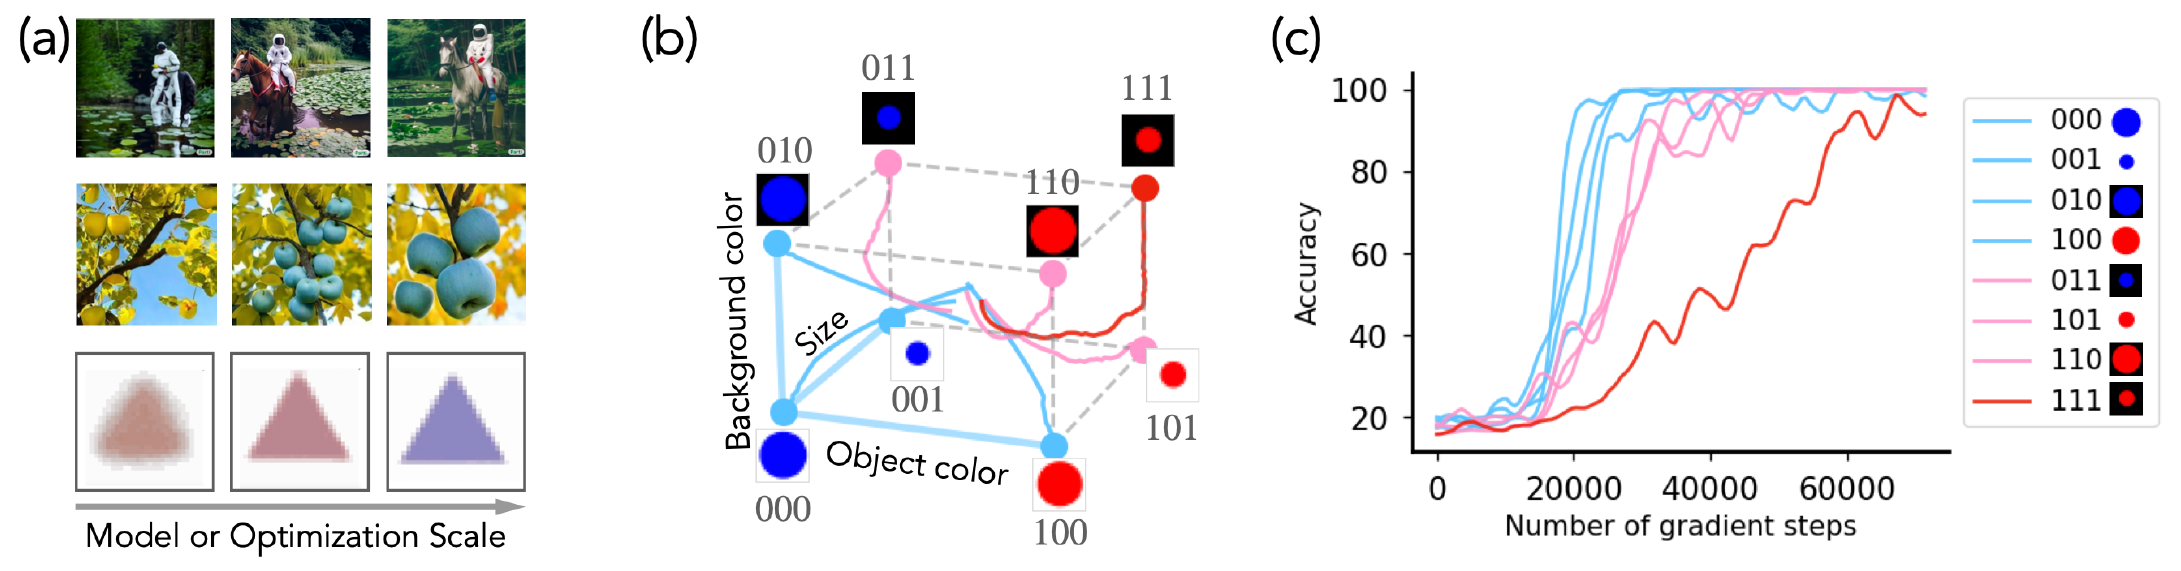
\includegraphics[width=0.9\linewidth]{figures/figure_1.png}
\end{figure}
% \end{textblock*}
\end{frame}

\begin{frame}[t]{Contributions}
     \begin{itemize}
        \item<1-3>Introduce \textit{Concept Space} to analyze a model’s learning
        \item<2-3>Show that \textit{Concept Signal} dictates the order of concept learning
        \item<3-3>Learning of concepts happens in two phases:
        \begin{itemize}
            \item (P1) learning of a hidden capability
            \item (P2) learning to generate the desired output from the input space
        \end{itemize}
     \end{itemize}
\end{frame}

% Hypothesis: generative models
% possess latent capabilities that are learned suddenly and consistently during training, but these
% capabilities are not immediately apparent since prompting the model via the input space may not elicit
% them

\begin{frame}[t]{Concept Space}
\begin{figure}
    \centering
    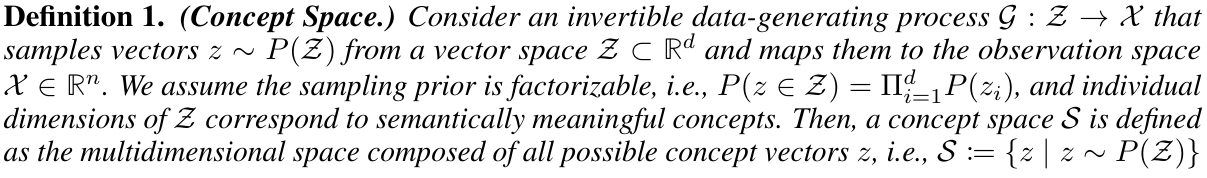
\includegraphics[width=0.77\linewidth]{figures/concept_space_def.png}
\end{figure}
\begin{figure}
    \centering
    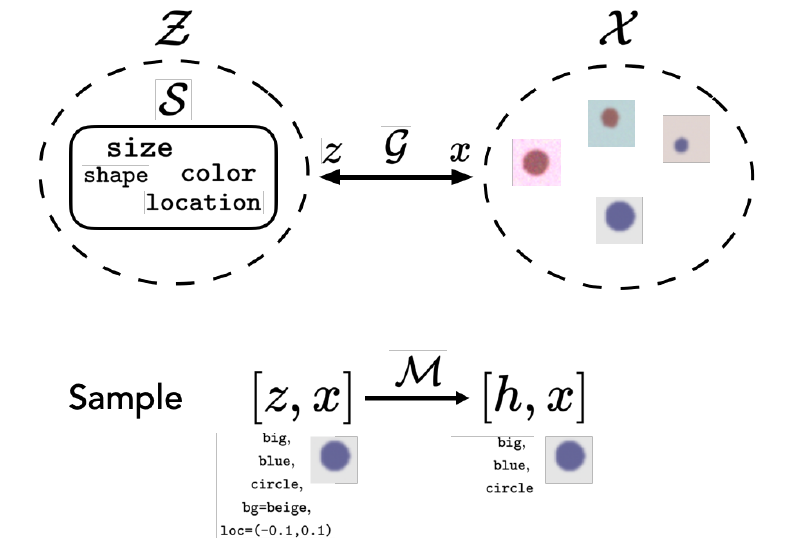
\includegraphics[width=0.38\linewidth]{figures/concept_space.png}
\end{figure}
\end{frame}

% using
% a mixing function M that yields conditioning information h := M(z), we can train a conditional
% generative model

\begin{frame}[t]{On Capability}
\begin{figure}
    \centering
    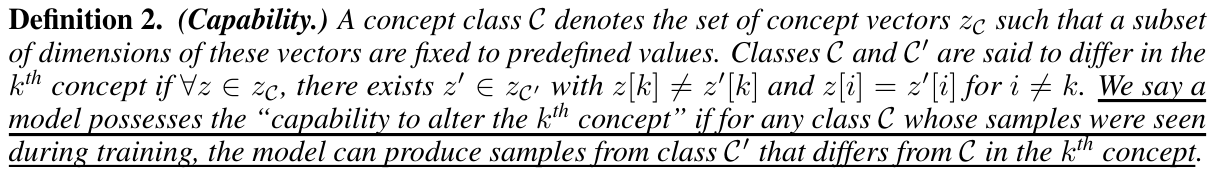
\includegraphics[width=0.77\linewidth]{figures/capability_def.png}
\end{figure}

\begin{itemize}
    \item we do not need to use the conditioning $h$ used for training
    \item other techniques can be used (over-prompting, latent interventions)
\end{itemize}
\end{frame}

\begin{frame}[t]{Concept Signal}
\begin{figure}
    \centering
    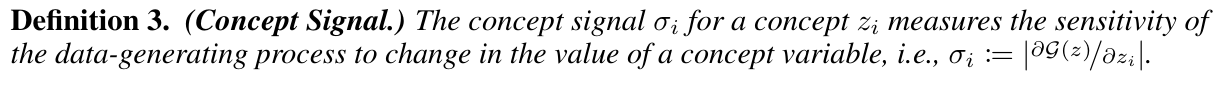
\includegraphics[width=0.77\linewidth]{figures/concept_signal_def.png}
    \end{figure}
    \quad Intuitively, concept signal indicates how much the model would benefit from learning a concept
    \begin{figure}
    \centering
    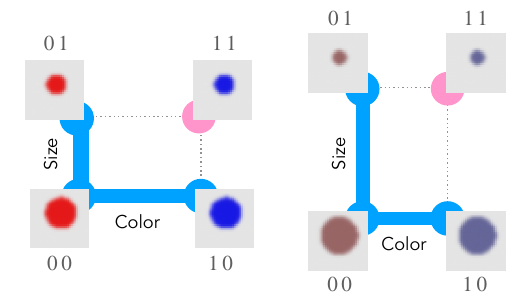
\includegraphics[width=0.49\linewidth]{figures/figure_2_concet_signal.png}
    \end{figure}
\end{frame}

\begin{frame}[t]{Experimental Setup}
\quad \textbf{Models:}
\begin{itemize}
    \item Variational Diffusion Model [1]
    \item Generate 3×32×32 (\& 3×64×64) images conditioned on $h$
\end{itemize}

\quad \textbf{Datasets:}
\begin{itemize}
    \item Synthetic toy 2D objects with controlled concepts
    \item CelebA
\end{itemize}

\quad \textbf{Evaluation:}
\begin{itemize}
    \item Classifier probes for individual concepts (U-Net)
    \item Using same training set
\end{itemize}
\end{frame}

% Evaluation Metric. To assess whether a generated image matches the desired concept class without
% human intervention, we follow literature on disentangled representation learning and train classifier probes for individual concepts using the diffusion model’s training data.
% U-Net [95] followed by an average pooling layer and n MLP
% classification heads for the n concept variables

\begin{frame}[t]{Concept Signal Determines Learning Speed}
\begin{columns}
\column{0.5\textwidth}
\begin{itemize}
    \item Changing the level of concept signal in the training data
    \item $h := z$
    \item speed of learning: inverse of the number of gradient steps required to reach 80\% accuracy on OOD class
\end{itemize}
\column{0.5\textwidth}
\begin{figure}
    \centering
    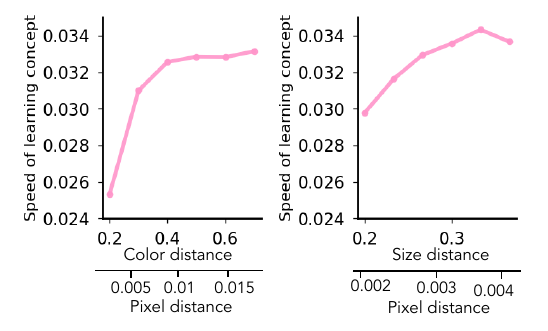
\includegraphics[width=\linewidth]{figures/figure_3_speed.png}
\end{figure}
\end{columns}
\end{frame}

\begin{frame}[t]{Concept Signal Governs Generalization Dynamics}
\begin{columns}
\column{0.4\textwidth}
\begin{itemize}
    \item Concept memorization: OOD generations biased towards class with strongest concept signal
    \item Problem when early stopping text-to-image models
    \item Unseen conditioning associated to nearest concept class
\end{itemize}
\column{0.6\textwidth}
\begin{figure}
    \centering
    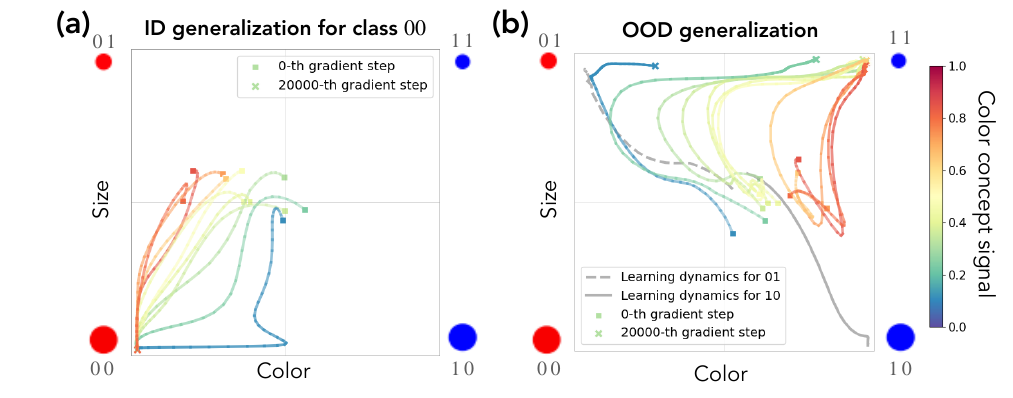
\includegraphics[width=\linewidth]{figures/figure_4.png}
\end{figure}
\end{columns}
\end{frame}

\begin{frame}[t]{Landscape Theory of Learning Dynamics}
\begin{columns}
\column{0.5\textwidth}
\begin{itemize}
    \item There is a sudden turn from concept memorization to OOD generalization
    \item Learning dynamics can be decomposed into two stages
    \item \textit{Hypothesis:} there is a phase change, in which the model learns to alter concepts
\end{itemize}
\column{0.5\textwidth}
\begin{figure}
    \centering
    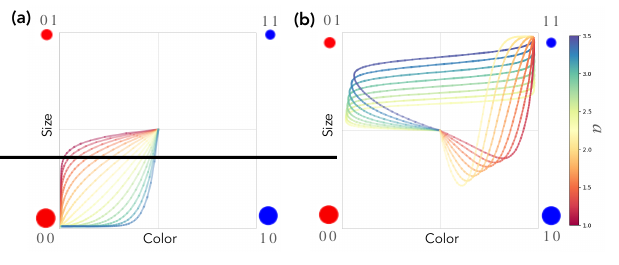
\includegraphics[width=\linewidth]{figures/figure_5.png}
\end{figure}
\end{columns}
\end{frame}

\begin{frame}[t]{Sudden Transitions in Learning Dynamics}
\begin{itemize}
    \item There is a phase in which the model is capable of disentangling concepts, but still produces incorrect images
    \item Naive input prompting is insufficient to elicit these capabilities and generate samples from \\OOD classes
    \item Second phase in learning dynamics: an
alignment between the input space and concept representations is learned
\end{itemize}
\end{frame}

\begin{frame}[t]{Different Guidance Scales}
\begin{figure}
    \centering
    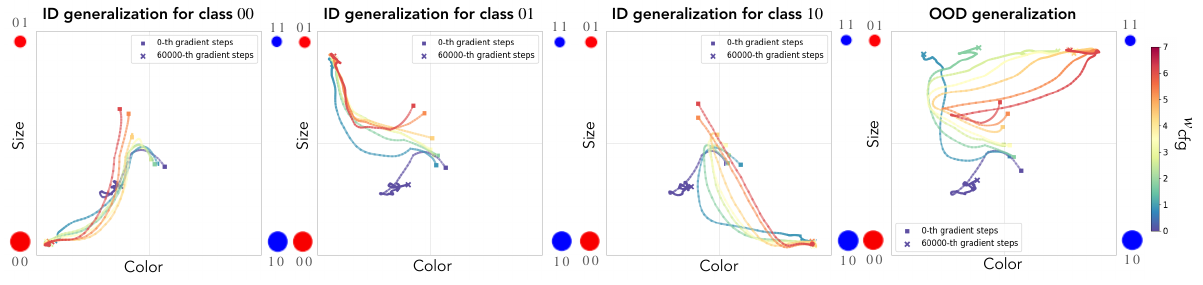
\includegraphics[width=0.92\linewidth]{figures/cfg.png}
\end{figure}
\end{frame}

\begin{frame}[t]{Techniques to elicit hidden capabilities}
\begin{enumerate}
    \item \textbf{Activation Space:} \textit{Linear Latent Intervention}
    \item \textbf{Input Space:} \textit{Overprompting}
\end{enumerate}
\begin{figure}
    \centering
    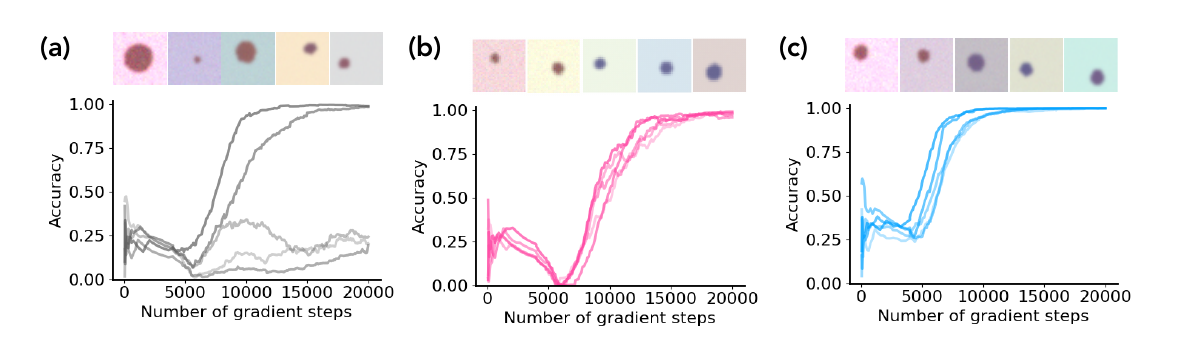
\includegraphics[width=0.7\linewidth]{figures/figure_6.png}
\end{figure}
\end{frame}

% Two techniques: \textit{figure_6}
% 1. Activation Space: Linear Latent Intervention. Given conditioning vectors h, during inference
% we add or subtract components that correspond to specific concepts (e.g., hblue ).
% 2. Input Space: Overprompting. We simply enhance the color conditioning to values of higher
% magnitude, e.g. (r, g, b) = (0.4, 0.4, 0.6) to (0.3, 0.3, 0.7).

% the model can consistently elicit the desired outputs much earlier than input prompting
% approximately the same number of gradient steps, irrespective of the seed, and that this is precisely
% the point of sudden turn in the learning dynamics in Fig. 4!

\begin{frame}[t]{Patching Embeddings}
\begin{enumerate}
    \item Take the embedding module from final checkpoint
    \item Patch it to an intermediate U-Net checkpoint
    \item Naive prompting works as well as previous techniques
\end{enumerate}

\begin{figure}
    \centering
    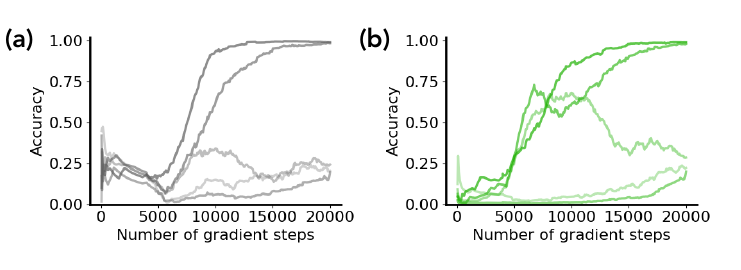
\includegraphics[width=0.5\linewidth]{figures/patching.png}
\end{figure}
\begin{itemize}
    \item \textit{Second phase aligns input space to intermediate representations}
    \item \textit{Embedding module disentangles concepts}
    \item \textit{U-Net generates a representation for each}
\end{itemize}
\end{frame}

\begin{frame}[t]{Results on CelebA}

\begin{figure}
    \centering
    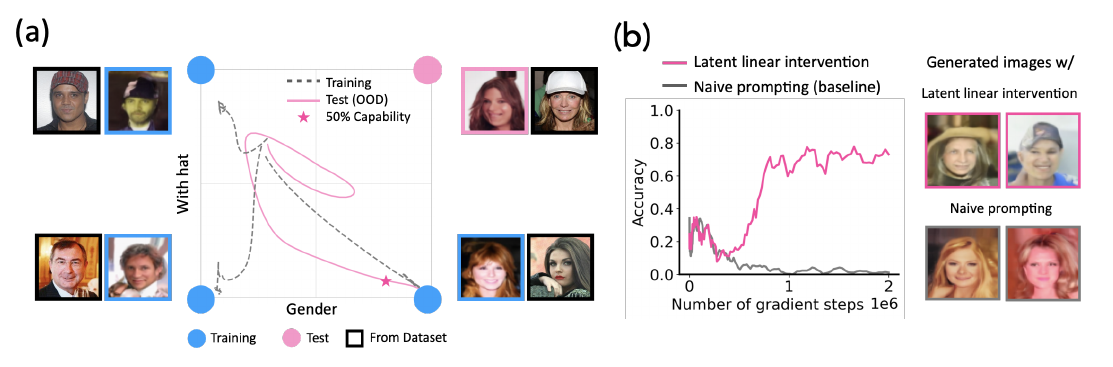
\includegraphics[width=0.95\linewidth]{figures/celeba.png}
\end{figure}
\end{frame}

\begin{frame}[t]{Effect of Underspecification}
\qquad In the previous experiments $h := z$, \textit{what if not?}
\begin{figure}
    \centering
    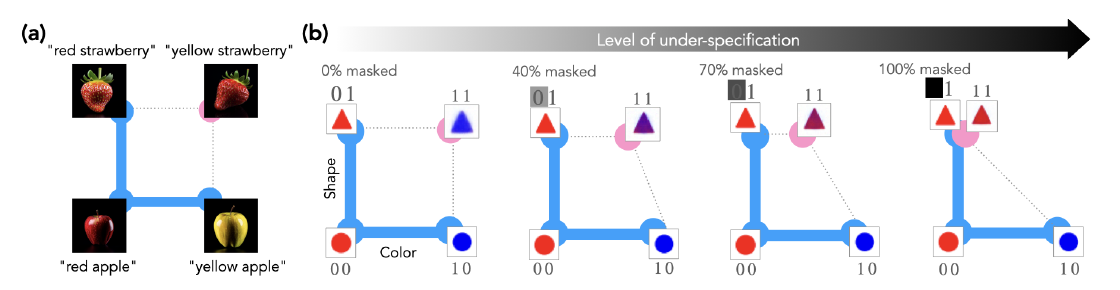
\includegraphics[width=0.8\linewidth]{figures/figure_9.png}
    \caption{Images of a strawberry are
often correlated with the color red}
\end{figure}
\begin{itemize}
    \item Simulate underspecification by randomly masking (e.g. \sout{red} triangle)
\end{itemize}
\end{frame}

\begin{frame}[t]{Underspecification hinders OOD generalization}
\begin{figure}
    \centering
    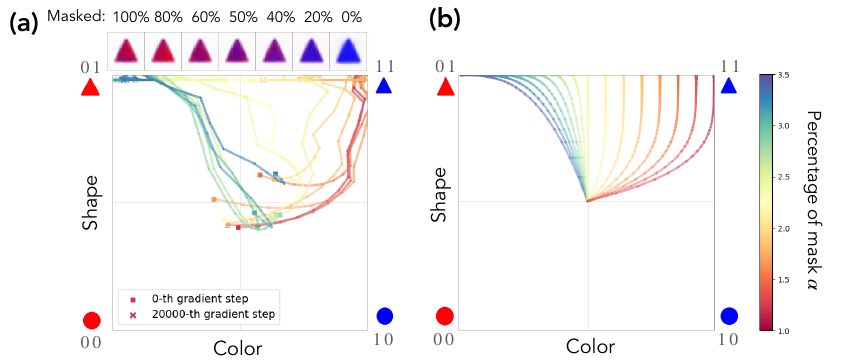
\includegraphics[width=0.65\linewidth]{figures/figure_10.png}
\end{figure}
\qquad When prompts are masked, the model’s understanding of shape triangle becomes intertwined
\\ \qquad
with color red, \textbf{even when blue is specified}
\end{frame}

\begin{frame}[t]{Overprompting and Underspecification}
\begin{figure}
    \centering
    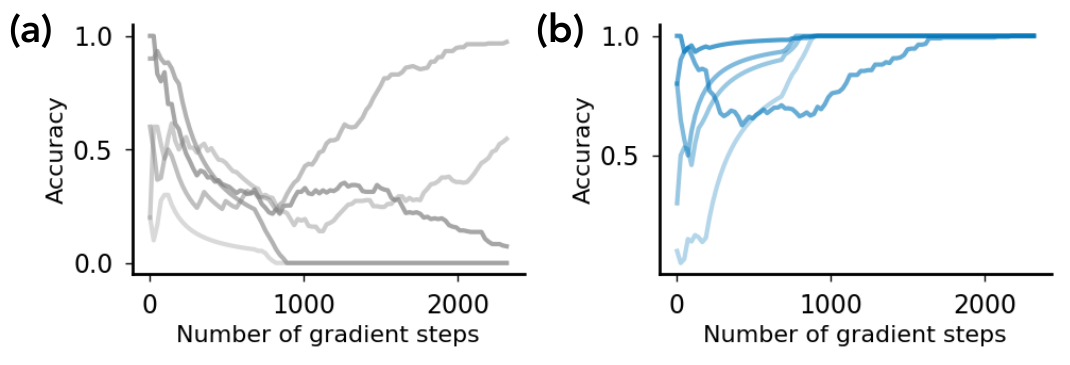
\includegraphics[width=0.65\linewidth]{figures/figure_11.png}
\end{figure}
\qquad Capability can develop prior to observable
behavior, \\ \qquad even in cases of underspecification.
\end{frame}

\begin{frame}{Conclusion}
    \begin{itemize}
        \item Concept Space may be useful to understand learning in generative models
        \item Concept Signal Dictates Speed of Learning
        \item Generative models learn to manipulate concepts earlier than exhibited
    \end{itemize}

\quad \textbf{Limitations:}
\begin{itemize}
    \item Real-world data are more complex (not always compositional)
    \item Concepts are not always linearly embedded in the vector space $\mathcal{Z}$
\end{itemize}
\end{frame}

\begin{frame}{References}
    [1] Diederik P. Kingma, Tim Salimans, Ben Poole, and Jonathan Ho. Variational diffusion models, NeurIPS 2021
    \hfill \break
\end{frame}

\end{document}